\chapter{Introdução ao teste automatizado com ênfase nos tipos de testes}
\label{cap:Introdução ao teste automatizado com ênfase nos tipos de testes}

\section{Conceito sobre Testes Automatizados}
\label{sec:Conceito sobre Testes Automatizados}
	
	A área de teste de software tem crescido bastante nos últimos anos pelo fato de ter um aumento nas pesquisas e profissionais da área de teste de software. Esse aumento tem a ver com o crescimento rápido dos software e a exigência da entrega de software com menos problemas e mais qualidade \cite{LivroAutomatizacao}.
    
    O teste de software tem como proposta mostrar que o software desenvolvido faz oque foi prometido fazer e serve também para encontrar problemas antes do software ser utilizado pelo usuário final\cite{EngSofSommerville}. Alem disso, os testes feitos em um software não implica que o mesmo se encontra livre de problemas ou o software vai agir de acordo com as especificações feitas em qualquer momento \cite{EngSofSommerville}.
    
    Os testes automatizados são testes que são executado por uma ferramenta que contém vários item de teste. Onde esses testes são executados por meio do controladores de testes, que é um modulo de software que invoca um módulo sob teste. Além do mais, fica promovendo entradas de testes, monitorando a execução do teste ,controlando o mesmo e por fim, relata os resultados \cite{EngdeSoftwareFMP}.
    
    As vantagens de se usar os testes automatizado, são a economia do tempo que teria caso o teste fosse feito de forma manual e  diminui os problemas que são encontrado durante o desenvolvimento do sistema \cite{LivroAutomatizacao}. Por causa desse motivo, o teste automatizado é considerado indispensável nos dias de hoje para o desenvolvimento, pois só ele executam vários teste com grande volume de forma confiável para assim poder agilizar essa atividade \cite{EngdeSoftwareFMP}.  
    
    O código de teste que é criado para fazer os testes automatizado é semelhante ao codigo de uma aplicação, sendo algumas vezes superior. Além do mais esse codigo de teste tem que ser confiável, pelo motivo que vai ser utilizado para fazer os testes \cite{EngdeSoftwareFMP}. 
    
    A automatização dos testes não são totalmente automatizado uma vez que só testa aquilo que foi planejado. Por outro lado, oque os testes automatizados não fazem é testar como as coisas estão ,exemplo seria a interface do sistema \cite{EngSofSommerville}.
    
    
    
    
	Na Figura 1 encontram-se os tipos de testes usados quando se quer implementar um teste automatizado no seu software.  
    \begin{figure}[h!]
	\centering
		\Caption{\label{fig:Sequencia_de_Testes} Testes }	
		\UNIFORfig{}{
			\fbox{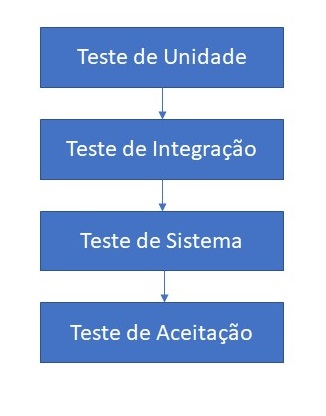
\includegraphics[width=8cm]{figuras/Sequencia_de_Testes.jpg}}
		}
       	{
			\Fonte{Elaborado pelo autor}
		}	
	\end{figure}
    
\subsection{Teste de unidade}
\label{sec:Teste de unidade}
	O teste de unidade é executado em todo o ciclo de vida do desenvolvimento do software, onde é testados as menores unidades componentes do sistema que são considerados: as classes, as funções e objetos do sistema. Onde se considera a performance do sistema e a lógica do usada no sistema. Nesse testes se usasse de parâmetros diferentes de entrada, para mostrar a existência do erro em cada componentes do sistema testado. Além disso, o teste de unidade pode ser usado como técnica para teste de caixa preta e caixa branca. No qual o teste de caixa preta pode ser aplicado na fase de desenvolvimento, mas o teste de caixa branca é o teste mais frequente a ser utilizado. \cite{ReginaldoRe} 
    
    Quando é executado o teste de unidade nas classes de objetos, os testes devem ser projetados para garantir a abrangência de todas as características do objeto \cite{EngSofSommerville}. Segundo o \cite{EngSofSommerville} deve-se "Testar todas as operações associadas ao objeto; Definir e verificar o valor de todos os atributos associados ao objeto; Colocar o objeto em todos os estados possíveis, oque significa simular todos os eventos que causam mudanças de estado;".
    
    %A herança, nas classes de objetos, é considerada complexa quando submetido a um teste de unidade. Pelo motivo de que, quando é testado uma operação na classe principal não se pode assumir que essa operação vai funcionar correto nas subclasses que herdaram essa operação. Por causa disso, é indispensável testar as operações nas subclasses que herdaram essa operação para todos os testes dessa operação\cite{EngSofSommerville}.
    
    %O testes de unidade automatizados são executado com o uso de \textit{framework} para testes(como JUnit, Selenion...), onde se desenvolve scripts que tem classes de testes genéricas ou pode ter classes de testes especificas, que quando executadas os testes criados nos scripts é informado por uma interfase gráfica se os testes deram certo ou deram errado. Com um conjunto de scripts de teste sendo executado em um \textit{framework}, o tempo para executar os testes pode ser em pouco segundo.\cite{EngSofSommerville}
    
    %Com o uso de ferramentas como JUnit, o desenvolvimento das classes de teste fica mais simples de implementar e executar os testes que foram pedidos. Contudo, existe um grande desafio em implementar as classes de testes, pelo fato de exigir um conhecimento de programação e de testes. \cite{UsingRulestoSupportSoftwareTesting}  
    
    


\subsection{Teste de integração}
\label{sec:Teste de integração}
	O teste de integração tem como definição um teste que verifica os componentes do sistema e testa cada um dos componentes. \cite{EngdeSoftwareFMP}. Onde verifica problemas envolvendo a construção do software. Consequentemente é uma técnica sistemática para a construção da arquitetura do software, onde simultaneamente realia os testes para encontrar problemas relacionados as interfaces do sistema \cite{pressman}.
    
    
    Dentro do teste de integração existem duas estrategias que são "bottom-up" e "top-down". Onde o "bottom-up" baseia-se em testar os módulos de baixo nível até chegar nos módulos de alto nível e o "top-down" é o inverso do "bottom-up" \cite{CidinhaCostaGouveia}.
	
    A estratégia top-down aborda a construção da arquitetura do software de forma incremental, onde os módulos são integrados e move-se para baixo por meio de uma hierarquia de controle que é iniciado com o módulo de controle principal. Os módulos subordinados ao módulo de controle principal são agregados de duas possíveis  formas na estrutura de hierarquia de controle: depth-first(primeiro-em-profundidade), onde faz a integração em todos os componentes criando um caminho de controle principal na estrutura do programa e breadth-first(primeiro-em-largura), onde junta todos os componentes subordinados a cada nível e move esses componentes através da estrutura horizontalmente. \cite{pressman}.
    
    Já a estratégia bottom-up aborda o inicio da construção e o teste com os módulos atômicos( nível mais baixo da estrutura do sistema). Onde os componentes são constituídos de baixo para cima, com isso proporciona o componentes subordinados a certos niveis estarem sempre disponíveis e a exigência de pseudocontroladores não vai existir \cite{pressman}.
   
    Quando o teste de integração é realizado, existe a possibilidade de que o mesmo afete o teste de unidade e o  também afete o custo dos testes. Por causa dos erros encontrados durante o teste de integração, pode provocar correções nas unidades testadas no teste de unidade. Onde vai implicar na correção da unidade e em um novo uso dos teste de unidade e de integração. Portando o teste de integração deve ser usado no começo do desenvolvimento junto com o teste de unidade. Se usando disso, ajuda a conter os custo de manutenção nas fases finais do desenvolvimento e contribui para o melhoramento da qualidade dos testes de unidade. \cite{MARLLOSPAIVAPRADO} 
    
    
    
    
\subsection{Teste de sistema}
\label{sec:Teste de sistema}
	O teste de sistema tem como foco verificar todo o sistema, para confirmar se todos os requisitos do software foi feito de forma correta. Onde nesse teste, é considerado todos as funcionalidades que são importante para o funcionamento do sistema, como : segurança, performance e robustez\cite{LivroAutomatizacao}.
    Acrescentando-se que, esse teste precisa aprovar os requisitos funcionas do software e  também precisa validar os requisitos não funcionais que foram estabelecidos \cite{ReginaldoRe}. Ademais esse teste aprova o sistema quando ele é integrado a um sistema maior \cite{pressman}.
    

    

    
    
    
    
    
\subsection{Teste de aceitação}
\label{sec:Teste de aceitação}
	O teste de aceitação é executado junto com o cliente com ou não supervisão dos desenvolvedores. Alem disso nesse teste, todo o sistema é testado pelo cliente para verificar a existência de erros. Após o teste, o cliente relata aos desenvolvedores os error que foram tidos no teste\cite{LivroAutomatizacao}. 
    Além do mais, esse teste é para garantir que o software cumpra todos os requistos funcionais, comportamentais e de desempenho estalecidos \cite{pressman}.
    
    Acrescentando-se que esse teste pode ser feito em um períodos longos (semanas ou meses), para assim descobrir erros cumulativos, que podem prejudicam o sistema \cite{pressman}. 
    
    
    
    


\chapter{Introdução a ferramenta BPMS com ênfase em sua arquitetura}
\label{cap:Introdução a ferramenta BPMS com ênfase em sua arquitetura}
Como mencionado antes uma ferramenta BPMS suporta as notações do BPMN e tem as disciplinas gerenciais do BPM dentro da ferramenta. A ferramenta BPMS tem origem em ferramentas de workflow que foram evoluindo ao longo do tempo, onde houve a junção de motores de regras de negocio e geração de aplicação na ferramenta de workflow. Assim as aplicações criadas dentro do BPMS são geradas e acessas por dentro do BPMS\cite{CBOK}.

O BPMS criou um nível de automação que possibilitou a junção dos modelos de negócios com regras e as informações que tem nas atividades do processo. Além disso,a ferramenta possou capacidade de gerir e criar aplicações somente como os modelos junto com as suas regras. Assim oferecendo um gerenciamento do fluxo do trabalho\cite{CBOK}.

As ferramentas BPMS dificilmente são parecidas, já que elas envolve diferentes etapas do ciclo de vida do BPM: onde os sistemas mais simples só envolver a parte de design dos processos e a automação do mesmo, já os sistemas mais complexo tem oque o sistema simples tem e contem o SOA, integrações com sistema de terceiros, Processamento de Eventos (CEP) e por fim, inteligencia do processo \cite{ProcessAwareBPM}.

Com o uso do SOA(Service-oriented architecture) ajudou os BPMS a fazerem integrações com os sistemas legados, onde o SOA é uma adaptador junto com web services para se comunicar com sistemas legados. Os BPMS utilizam-se dessa arquitetura para se comunicar com os outros sistemas das organizações e assim tirando proveito dessa camada nos processos criados \cite{CBOK}.

Devido a competição entre fornecedores, ocorre uma evolução dos BPMS e consequentemente, uma corrida para fornecer o melhor ambiente para a operação, conduzindo assim uma rápida expansão de sua capacidade e melhoria geral de sua qualidade e estabilidade, essa evolução direciona-se em duas categorias. As ferramentas autônomas, que por seu custo mais baixo, facilita às organizações, a capacidade de análise e definição de seus processos e fluxos de trabalho, assim como análise de regras de negócio, e muitas vezes, a descoberta de inconsistências e conflitos. Outra categoria consiste nos grupos integrados de ferramentas, que evoluíram para a geração de aplicações capazes de prover suporte à lógica complexa e transações em alto volume \cite{CBOK}.


\section{Arquitetura do BPMS}
\label{sec:Arquitetura do BPMS}
	Na Figura a baixo podemos ver como é divido a Arquitetura de uma ferramenta BPMS
    
\begin{figure}[h!]
	\centering
		\Caption{\label{fig:SOA} Arquitetura do BPMS }	
		\UNIFORfig{}{
			\fbox{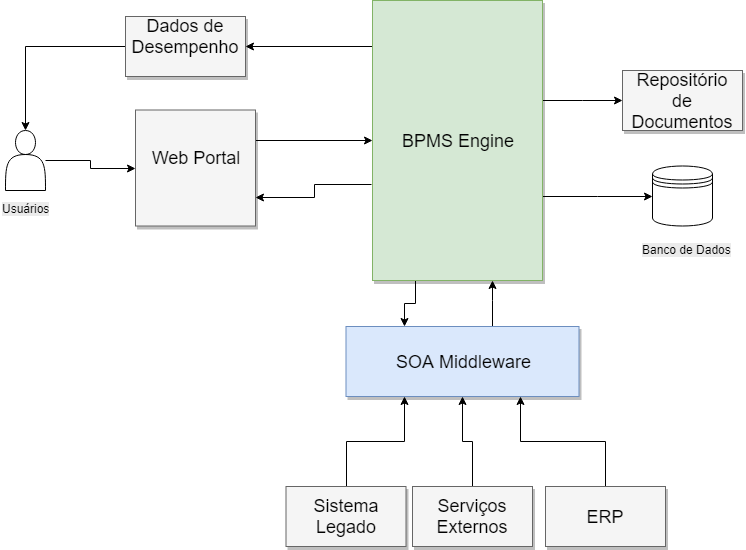
\includegraphics[width=15cm]{figuras/BPMS__Arquitetura.png}}
		}
       	{
			\Fonte{Elaborado pelo autor}
		}	
	\end{figure}
    
    \textbf{BPMS Engine }: considerado o coração do BPMS, é a parte do BPMS que tem diferentes funcionalidades que podem ser a seguintes: criação de processos executáveis (Cases), distribuição das atividades para os participantes do processo, capacidade de recuperar e guardar os dados necessários para executar o processo, executar atividades automatizadas para diferente tipos de software, criação e modificação de modelos de processos, criação do modelo de dados usado nos processos, capacidade de criar formulários e mantém o controle das atividades que estão perto de terminar o tempo.   \cite{ProcessAwareBPM}.
    
    \textbf{SOA Middleware}: é uma middleware que é usado no desenvolvimento de aplicações e integrações com diferentes tipos de sistemas \cite{CBOK}. O SOA se conecta com diferentes serviços para obter dados requerido pelo processo na aplicação BPMS.
    
    \textbf{Web Portal}: Portal que mostra ao usuário quando o mesmo entra na aplicação. Nesse portal o usuário poderá: criar cases(instância de um processo), fazer buscas e administrar os processo.  
    
    %é um conjunto flexível de princípios de desenho de infraestrutura usados no desenvolvimento de aplicações e integração de sistemas.
    



%	\begin{figure}[h!]
%		\centering		\Caption{\label{fig:}  }	
%		\UNIFORfig{}{
%			\fbox{\includegraphics[width=8cm]{figuras/}}
%		}{
%			\Fonte{}			
%		}	
%	\end{figure}















